\documentclass[tikz,border=2pt]{standalone}
\usepackage{amsmath,amssymb}
\usepackage{tikz}
\usetikzlibrary{arrows.meta}

\begin{document}
% If det Df(x_0) != 0, a small neighbourhood of x_0 is mapped bijectively onto a neighbourhood
% of y_0 = f(x_0), with a C^1 inverse whose derivative is the inverse matrix.
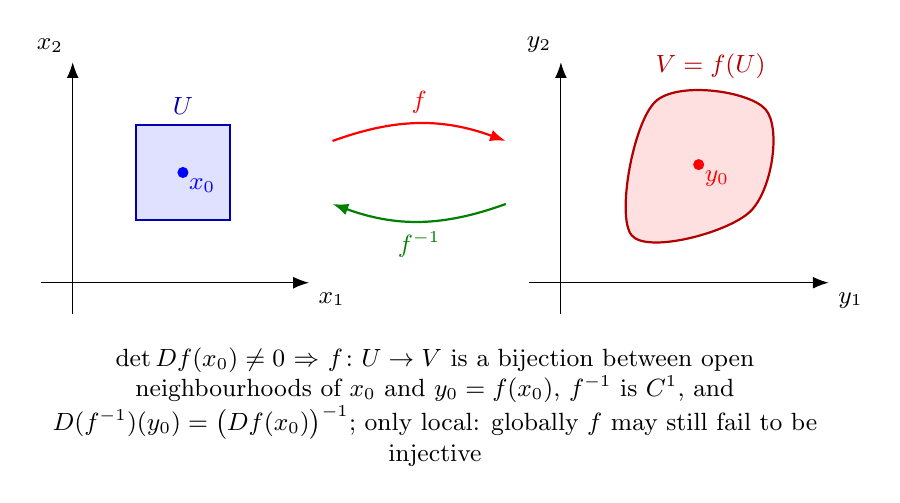
\begin{tikzpicture}[every node/.style={font=\small}, >={Latex[length=2mm]}]
	\draw[->] (-0.4,0) -- (3.0,0) node[below right, font=\small] {$x_1$};
	\draw[->] (0,-0.4) -- (0,2.8) node[above left, font=\small] {$x_2$};
	\fill[blue!12] (0.8,0.8) rectangle (2.0,2.0);
	\draw[blue!70!black, thick] (0.8,0.8) rectangle (2.0,2.0);
	\fill[blue] (1.4,1.4) circle (2pt) node[below right, inner sep=2pt, font=\small] {$x_0$};
	\node[blue!70!black, font=\small] at (1.4,2.25) {$U$};
	\draw[->, thick, red] (3.3,1.8) to[bend left=20] node[midway, above] {$f$} (5.5,1.8);
	\draw[->, thick, green!50!black] (5.5,1.0) to[bend left=20] node[midway, below] {$f^{-1}$} (3.3,1.0);
	\begin{scope}[xshift=6.2cm]
		\draw[->] (-0.4,0) -- (3.4,0) node[below right, font=\small] {$y_1$};
		\draw[->] (0,-0.4) -- (0,2.8) node[above left, font=\small] {$y_2$};
		\fill[red!12] plot[smooth cycle, tension=0.6] coordinates {(0.9,0.6) (2.4,0.9) (2.6,2.2) (1.2,2.3)};
		\draw[red!70!black, thick] plot[smooth cycle, tension=0.6] coordinates {(0.9,0.6) (2.4,0.9) (2.6,2.2) (1.2,2.3)};
		\fill[red] (1.75,1.5) circle (2pt) node[below right, inner sep=2pt, font=\small] {$y_0$};
		\node[red!70!black, font=\small] at (1.9,2.75) {$V=f(U)$};
	\end{scope}
	\node[anchor=north, align=flush center, text width=10cm] at (4.6,-0.7) {$\det Df(x_0)\neq0$ $\Rightarrow$ $f\colon U\to V$ is a bijection between open neighbourhoods of $x_0$ and $y_0=f(x_0)$, $f^{-1}$ is $C^1$, and $D(f^{-1})(y_0)=\big(Df(x_0)\big)^{-1}$; only local: globally $f$ may still fail to be injective};
\end{tikzpicture}
\end{document}
